\documentclass[border=10pt]{standalone}
\usepackage[svgnames]{xcolor}
\usepackage{amsmath}
\usepackage{pgfplots}
\pgfplotsset{compat=newest}
\usepackage[sfdefault]{FiraSans}
\usepackage{FiraMono}
\renewcommand*\familydefault{\sfdefault}
\begin{document}
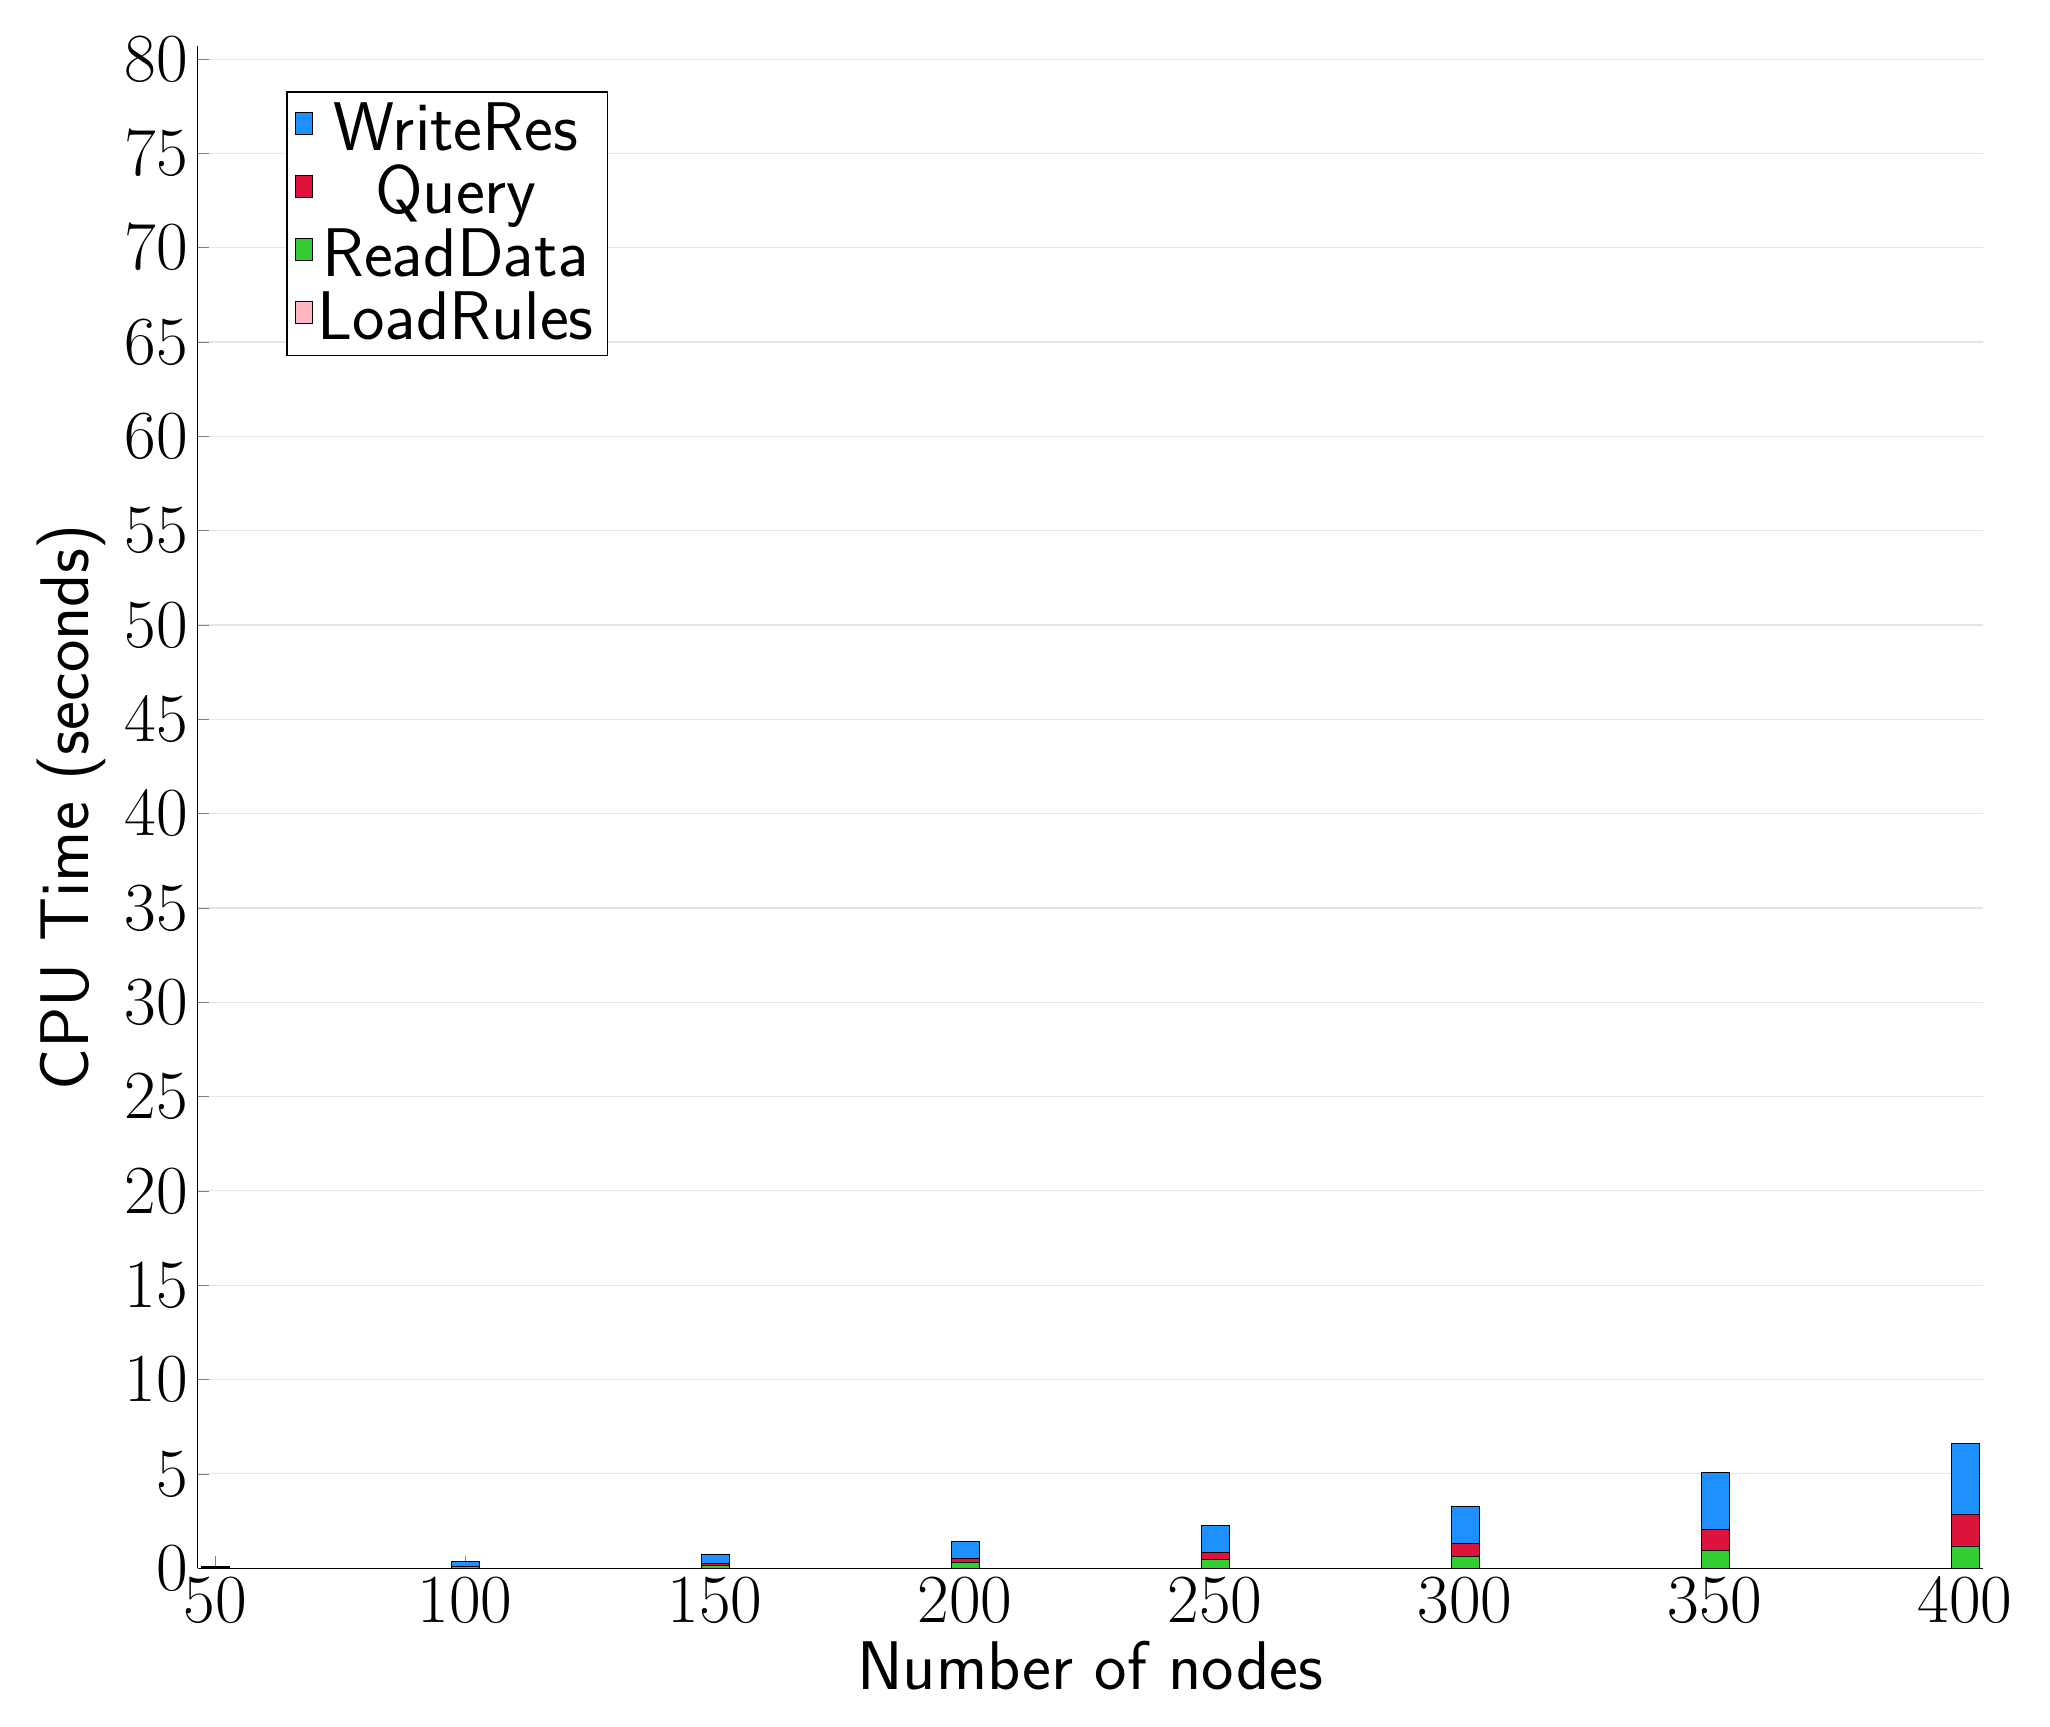
\begin{tikzpicture}
\begin{axis}[
   ybar stacked,
   width=2\textwidth,
   bar width=0.35cm,
   ymajorgrids, tick align=inside,
   major grid style={draw=gray!20},
   xtick=data,
   ymin=0, ymax=80.70666666577259,
   axis x line*=bottom,
   axis y line*=left,
   enlarge x limits=0.01,
   legend style={
       at={(0.23, 0.97)},
       anchor=north east,
       legend columns=1,
       font=\Huge,
   },
   ylabel={CPU Time (seconds)},
   xlabel={Number of nodes},
   label style={font=\Huge},
   tick label style={font=\Huge},
]
\addlegendimage{fill=DodgerBlue, draw=black, line width=0.2pt}
\addlegendentry{WriteRes}
\addlegendimage{fill=Crimson, draw=black, line width=0.2pt}
\addlegendentry{Query}
\addlegendimage{fill=LimeGreen, draw=black, line width=0.2pt}
\addlegendentry{ReadData}
\addlegendimage{fill=LightPink, draw=black, line width=0.2pt}
\addlegendentry{LoadRules}
\addplot +[fill=LightPink, draw=black, line width=0.2pt] coordinates {
(50, 0.0027663333333333338)
(100, 0.0059529999999999965)
(150, 0.0033749999999999995)
(200, 0.004127666666666667)
(250, 0.00438433333333333)
(300, 0.00404633333333333)
(350, 0.0045093333333333365)
(400, 0.0038996666666666637)
};
\addplot +[fill=LimeGreen, draw=black, line width=0.2pt] coordinates {
(50, 0.019910666666666667)
(100, 0.08723233333333334)
(150, 0.15247733333333333)
(200, 0.3099403333333333)
(250, 0.442143)
(300, 0.6132673333333333)
(350, 0.9574886666666668)
(400, 1.178814)
};
\addplot +[fill=Crimson, draw=black, line width=0.2pt] coordinates {
(50, 0.0032759999999999964)
(100, 0.028692333333333334)
(150, 0.08312466666666667)
(200, 0.19486100000000003)
(250, 0.380474)
(300, 0.7018733333333333)
(350, 1.0950486666666666)
(400, 1.6752976666666666)
};
\addplot +[fill=DodgerBlue, draw=black, line width=0.2pt] coordinates {
(50, 0.051947)
(100, 0.23057000000000002)
(150, 0.5140876666666666)
(200, 0.9286819999999999)
(250, 1.4531189999999998)
(300, 1.9822016666666666)
(350, 3.0218043333333333)
(400, 3.7561436666666665)
};
\end{axis}
\end{tikzpicture}

\end{document}
